\beginsong{Banner, Zelte}[wuw={Wolfgang Hartmann, VCP Stamm Franken, 1980er Jahre}, pfii={80}, pfiii={37}, gruen={170}, siru={27}]

\beginverse  
\endverse
\centering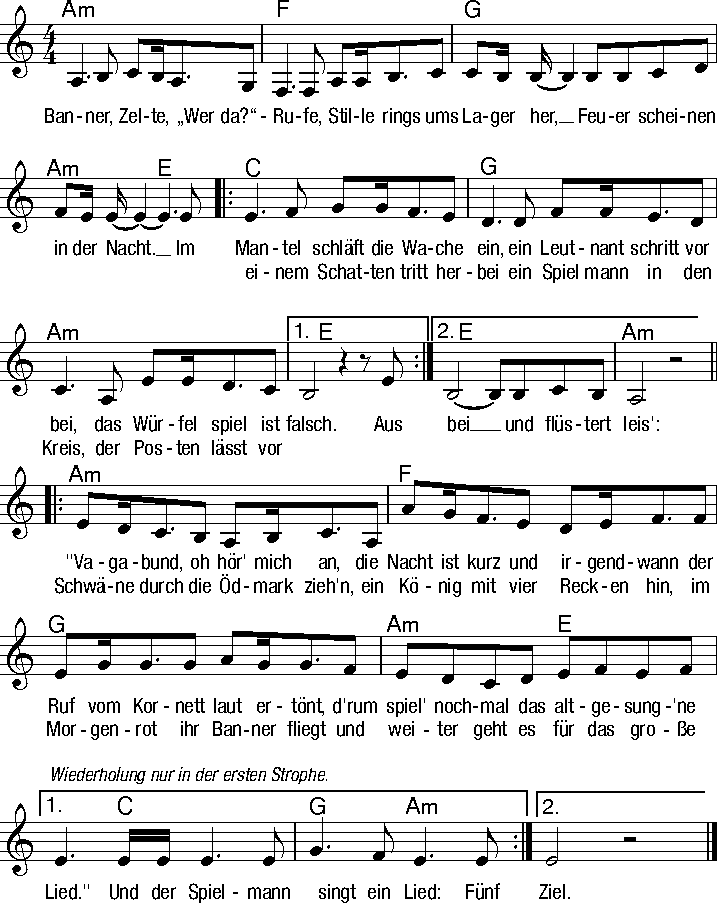
\includegraphics[width=1\textwidth]{Noten/Lied008.pdf}

\beginverse
\[Am]Im Feindeslager hört man's \[F]auch, durch Stille säuselt \[G]Melodie,
Herzen lauschen \[Am]wie noch nie. \[E]
Die \[C]Klampfe in der Hand, der \[G]Spielmann singt allein und 
\[Am]alles lauscht in dieser \[E]Nacht.
Doch \[C]plötzlich hinter sich hört \[G]er wie vereint den \[Am]Chor 
und alle stimmen \[E]ein in diese Melo\[Am]dei:
\endverse	

\beginchorus
'Fünf \[Am]Schwäne durch die Ödmark zieh'n, ein \[F]König mit vier Recken hin.
Im \[G]Morgenrot ihr Banner fliegt und \[Am]weiter geht es \[E]für das gute Ziel.'

Und \[Am]als der Morgen hell erstrahlt, die \[F]Schlacht beginnt, die Trommel warnt.
Vor\[G]ne steht ein Grenadier, er \[Am]denkt zurück und \[E]legt nieder das Schwert.
\endchorus
 
\beginverse
Und ^als drei Jahr' vergangen ^war'n, das Feld liegt öd und ^leer vorweg
und nichts erinnert ^mehr daran, ^
an ^eine nicht gewes'ne Sch^lacht, doch plötzlich hört man ^leis'
der Nachtigallen ^Schlag.
Als ^ob eine fremde Melo^die zög über das ^Land,
von Ferne weht ein ^Wind und trägt sie ^fort.
\endverse

\beginchorus
'Fünf Schwäne durch die Ödmark zieh'n, ein \[F]König mit vier Recken hin.
Im \[G]Morgenrot ihr Banner fliegt und \[Am]weiter geht es \[E]für das gute Ziel.' \[Am]
\endchorus

\endsong
